\begin{enumerate}[label=\tiny\purple{\faIcon{calculator}}]
  \item \textit{Grafos:}
        \parrafoDestacado{
          Un grafo $G$ es una terna $(V, E, \varphi)$, con $V$ un conjunto \blue{vértices},
          $E$ un conjunto \blue{aristas} y $\varphi$ es la función de incidencia.
        }
        La función $\varphi$ toma un elemento de $E$ y lo manda a un par formado por elementos de $V$.
        $$
          \varphi: E \to (v_i, v_j)  ~ \text{con} ~ v_i, v_j \en V
        $$
        $$
          \llave{rcl}{
            V & = & \set{v_1, \ldots, v_{\blue{n}}}\\
            E & = & \set{e_1, \ldots, e_{\magenta{m}}}
          }
        $$

  \item \textit{vértices o nodos adyacentes:}
        $$
          v \ytext w \en V, ~\text{si}~ \orange{e} = \ob{(v, w)}{\text{notación}\\\text{de aristas}} \en E
        $$
        donde el \textit{\ul{e}dge o arista} $\orange{e}$ es \ul{incidente} a $v$ y $w$.

  \item \textit{Vecindad, \ul{N}eighborhood:}

        Conjunto con los vértices adyacentes a $v$:
        $$
          N(v) = \set{w \en V : (v, w) \en E}.
        $$

  \item \textit{Multigrafo y Pseudografo:}

        En un \ul{multigrafo} puede haber más de una arista conectando el mismo par de vértices.
        Un \ul{pseudografo}  es un \ul{multigrafo} que también puede tener \textit{loops}.
        \tikzset{
          grafo local/.style={
              node distance = 3cm,
              nodo/.style={circle,
                  draw=violet,
                  fill=violet!5!white,
                  inner sep = 2pt,
                  thick,
                },
              arista/.style={ultra thin, bend left=30pt},
              arista2/.style={ultra thin, bend right=30pt},
              every node/.style={font={\tiny}},
              rulo/.style 2 args = {out=##1, in=##1+45, looseness=4, color={##2}},
            },
        }
        $$
          \begin{tikzpicture} [grafo local]
            \node[nodo] (v1) {$v_1$};
            \node[nodo, right of=v1] (v2) {$v_2$};
            \node[nodo, below right= 3cm of v1] (v3) {$v_3$};
            \node[nodo, below of = v1] (v4) {$v_4$};
            \draw[arista] (v1) to node[midway, above]{$e_{12} = (v_1, v_2)$} (v2);
            \draw[arista2] (v1) to node[midway, below]{$e_{12} = (v_1, v_2)$} (v2);
            \draw[] (v2) to node[midway, left]{$e_{23} = (v_2, v_3)$} (v3);
            \draw[arista] (v2) to node[midway, right]{$e_{23} = (v_2, v_3)$} (v3);
          \end{tikzpicture}
          \qquad
          \begin{tikzpicture} [ grafo local ]
            \node[nodo] (v1) {$v_1$};
            \node[nodo, right of=v1] (v2) {$v_2$};
            \node[nodo, below right= 3cm of v1] (v3) {$v_3$};
            \node[nodo, below of = v1] (v4) {$v_4$};
            \draw[arista] (v1) to node[midway, above]{$e_{12} = (v_1, v_2)$} (v2);
            \draw[arista2] (v1) to node[midway, below]{$e_{12} = (v_1, v_2)$} (v2);
            \draw[] (v2) to node[midway, left]{$e_{23} = (v_2, v_3)$} (v3);
            \draw[arista] (v2) to node[midway, right]{$e_{23} = (v_2, v_3)$} (v3);
            \draw[rulo={200}{Cerulean}] (v1) to node[midway, below]{$e_{11} = (v_1, v_1)$} (v1);
            \draw[rulo={250}{Cerulean}] (v3) to node[midway, below]{$e_{33} = (v_3, v_3)$} (v3)    ;
            \draw[rulo={250}{Cerulean}] (v4) to node[midway, below]{$e_{44} = (v_4, v_4)$} (v4)    ;
          \end{tikzpicture}
        $$

  \item \textit{Grado de un vértice, $d_G(v)$}:

        Es la cantidad de \textit{aristas} que tiene incidentes.
        $$
          \begin{tikzpicture} [ grafo style ]
            \node[nodo] (v1) {$v_1$};
            \node[nodo, right of=v1] (v2) {$v_2$};
            \node[nodo, below of=v2] (v3) {$v_3$};
            \node[nodo, left of=v3] (v4) {$v_4$};
            \node[nodo, above right of=v2] (v5) {$v_5$};
            \draw[] (v1) to (v2);
            \draw[] (v2) to (v3);
            \draw[] (v3) to (v4);
            \draw[] (v1) to (v4);
            \draw[] (v2) to (v5);
            \node[right  = 2cm of v2] (A) {$d_G(v_1) = d_G(v_4) = d_G(v_4) = 2$};
            \node[below =0.2cm of A] (B) {$d_G(v_2) = 3$};
            \node[below =0.2cm of B] (C) {$d_G(v_5) = 1$};
          \end{tikzpicture}
        $$

  \item \textit{Grafo Completo $K_n$:}
        Cuando todos los vértices son adyacentes entre sí.
        $$
          \begin{tikzpicture} [grafo style]
            \node[nodo] (v1) {$v_1$};
            \node[nodo, right of=v1] (v2) {$v_2$};
            \node[nodo, below of=v2] (v3) {$v_3$};
            \node[nodo, left of=v3] (v4) {$v_4$};
            \draw[] (v1) to (v2);
            \draw[] (v2) to (v3);
            \draw[] (v3) to (v4);
            \draw[] (v1) to (v4);
            \draw[] (v2) to (v4);
            \draw[] (v3) to (v1);
            \node[above = 0.2cm of v2] (A) {$K_4$};
          \end{tikzpicture}
          \qquad
          \begin{tikzpicture} [grafo style]
            \node[nodo] (v1) {$v_1$};
            \node[nodo, right of=v1] (v2) {$v_2$};
            \draw[] (v1) to (v2);
            \node[above = 0.2cm of v2] (B) {$K_2$};
          \end{tikzpicture}
        $$
        $$
          \cajaResultado{
            \text{
              Un grafo completo de $n$ vértices, $K_n$ tiene un total de $\frac{n \cdot (n-1)}{2}$ \textit{aristas}.
            }
          }
        $$

  \item \textit{Grafo complemento:}

        Dado $G = (V, E)$, el \textit{grafo complementario} $\bar{G} = (V, \bar{E})$, donde el conjunto $V$
        es igual en $G$ y $\bar{G}$ mientras que $E \inter \bar{E} = \vacio$.
        $$
          \begin{tikzpicture} [ grafo style ]
            \node[nodo] (v1) {$v_1$};
            \node[nodo, right of=v1] (v2) {$v_2$};
            \node[nodo, below of=v2] (v3) {$v_3$};
            \node[nodo, left of=v3] (v4) {$v_4$};
            \draw[] (v1) to (v2);
            \draw[] (v3) to (v4);
            \draw[] (v1) to (v4);
            \draw[] (v2) to (v4);
            \node[left = 0.5cm of v1] (G) {$G$};
          \end{tikzpicture}
          \qquad
          \qquad
          \begin{tikzpicture} [ grafo style ]
            \node[nodo] (v1) {$v_1$};
            \node[nodo, right of=v1] (v2) {$v_2$};
            \node[nodo, below of=v2] (v3) {$v_3$};
            \node[nodo, left of=v3] (v4) {$v_4$};
            \draw[] (v1) to (v3);
            \draw[] (v3) to (v2);
            \node[right = 0.5cm of v2] (Gcomp) {$\bar{G}$};
          \end{tikzpicture}
        $$
        Dado que $G \union \bar{G}$ hacen un \textit{grafo completo}:
        $$
          \cajaResultado{
            \text{
              Si $G$ tiene $n$ \textit{vértices} y $\red{m}$ \textit{aristas}
              $\bar{G}$ tendrá, $\frac{n \cdot (n - 1)}{2} - \red{m}$ \textit{aristas}.
            }
          }
        $$

  \item \hypertarget{teoria-3:recorridos}{\textit{Recorridos, caminos, circuitos, ciclos}}
        \begin{enumerate}[label=\faIcon{snowman}$_{\arabic*)}$]
          \item \textit{Recorrido o caminata (Walk)}:

                Secuencia alternada de vértices adyacentes y aristas. Nada raro. Se pueden repetir, vale todo.

          \item \textit{Camino (Path)}:

                Es un \textit{recorrido} que no pasa dos veces por el mismo vértice, en consecuencia
                tampoco repetís aristas.

          \item \textit{Senda o Rastro (Trail)}:

                Es un \textit{recorrido} que no repite aristas, pero podrías repetir vértices:
                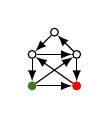
\begin{tikzpicture}
                  [
                    node distance = 0.4 cm,
                    nodo/.style={circle, draw=black, fill=gray!5!white, inner sep = 1pt},
                    arista/.style={-latex, thin},
                    baseline=-15,
                  ]
                  \node[nodo] (1) {};
                  \node[nodo, below left of = 1] (2) {};
                  \node[nodo, below right of = 1] (3) {};
                  \node[nodo, below of = 2, OliveGreen] (4) {};
                  \node[nodo, below of = 3, red] (5) {};
                  \draw[arista] (4) to (3) {};
                  \draw[arista] (3) to (1) {};
                  \draw[arista] (1) to (2) {};
                  \draw[arista] (2) to (3) {};
                  \draw[arista] (3) to (5) {};
                  \draw[arista] (5) to (2) {};
                  \draw[arista] (2) to (4) {};
                  \draw[arista] (4) to (5) {};
                \end{tikzpicture}

          \item \textit{Circuito (Circuit)}:

                Es una \textit{senda cerrada}, es decir empieza y terminar en el mismo vértice. Puede
                repetir vértices intermedio pero no repite aristas.

          \item \textit{Ciclo o Circuito simple}:

                Es una mezcla entre \textit{circuito} y \textit{\green{camino}} de 3 o más vértices
                que no repite vértices excepto por el primero y el último.
        \end{enumerate}

  \item \red{Di}grafos, grafos \red{Di}rigidos. Es un grafo con aristas \red{di}rigidas:
        \tikzset{
          digrafo style/.style={
              node distance = 3cm,
              nodo/.style={circle,
                  draw=violet,
                  fill=violet!5!white,
                  inner sep = 2pt,
                  thick
                },
              arista/.style={thin},
              arco/.style={-Stealth, thin, bend right=30pt},
              every node/.style={font={\small}},
              rulo/.style 2 args = {out=##1, in=##1+45, looseness=4, color={##2}},
            },
        }

        \begin{itemize}
          \item
                $D$ o  $G$: \textit{Digrafo:}

                Los \textit{vértices} se llaman \textit{arcos}, que van de
                $$
                  \begin{tikzpicture}[digrafo style]
                    \node[nodo, label={[above]{cola de $e$}}] (cola) {$u$};
                    \node[nodo, right of = cola, label={[above]{cabeza de $e$}}] (cabeza) {$w$};
                    \draw[arco] (cola) to node[midway, below]{$e = (u, w)$} (cabeza);
                  \end{tikzpicture}
                $$

          \item
                $d_{in}(v)$: \textit{Grado de entrada} de $v$.

                Cantidad de \textit{arcos} que llegan a $v$. Es la cantidad de \textit{arcos}
                que tienen a $v$ como cabeza.

          \item
                $d_{out}(v)$: \textit{Grado de entrada} de $v$.

                Cantidad de \textit{arcos} que salen de $v$. Es la cantidad de \textit{arcos}
                que tienen a $v$ como cola.

          \item
                \textit{grafo subyacente de un digrafo $D$:} Es el grafo $G^s$ que resulta de sacar las direcciones
                de los arcos.
                $$
                  \begin{tikzpicture}[digrafo style, baseline = 0]
                    \node[nodo] (cola) {$u$};
                    \node[nodo, right of = cola] (cabeza) {$w$};
                    \draw[arco] (cola) to  (cabeza);
                    \draw[arco] (cabeza) to  (cola);
                  \end{tikzpicture}
                  \quad\Entonces{convierto a grafo}[subyacente]\quad
                  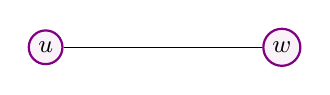
\begin{tikzpicture}[digrafo style, baseline = 0]
                    \node[nodo] (cola) {$u$};
                    \node[nodo, right of = cola] (cabeza) {$w$};
                    \draw[arista] (cola) to  (cabeza);
                  \end{tikzpicture}
                $$
        \end{itemize}

  \item \textit{Grafo bipartito:}
        \begin{center}
          Sea $G = (V,E)$ con $V = \set{v_1, \ldots, v_n}$ y $E = \set{e_1, \ldots, e_m}$

          $G$ es \textit{bipartito} $\sisolosi V = V_1 \union V_2$
          con
          $V_1 \distinto \vacio ~ \land ~ V_2 \distinto \vacio ~ \land ~ V_1 \inter V_2 = \vacio$

          $G$ es \textit{bipartito} $\sisolosi$ no tiene ciclos impares
        \end{center}
        Ejemplo:
        $$
          \begin{tikzpicture} [grafo style, node distance= 1cm]
            \node[nodo, purple] (1){$1$};
            \node[nodo, below of = 1, purple] (2){$2$};
            \node[nodo, below of = 2, purple] (3){$3$};
            \node[nodo, right =1cm of  1, OliveGreen] (4){$4$};
            \node[nodo, below  = 1cm of  4, OliveGreen] (5){$5$};
            \draw[arista, ultra thick]
            (1) to (4) to (3)
            (1) to (5) to (2);
            \node[compConexa, fit=(1)(3), inner sep = 10pt] {};
            \node[above left = 0.5cm of 1] (V1) {$V_1$} ;
            \node[compConexa, fit=(4)(5), inner sep = 10pt]{};
            \node[above right = 0.5cm of 4] (V2) {$V_2$} ;
            \node[very thick, draw = Cerulean, dotted, fit=(V1)(V2)(3)(5), inner sep = 15pt] (V){};
            \node[above right = 0.2cm of V] (V) {$V$} ;
          \end{tikzpicture}
        $$
        \parrafoDestacado[\atencion]{
          En un grafo \textit{bipartito} se pueden armar dos bandos, donde no hay \textit{friendly fire}.
        }

  \item \textit{Grafo subyacente o Subgrafo:}
        \begin{center}
          Dado un grafo $G = (V, E)$, se denomina \textit{subgrafo} al grafo

          $G' = (V', E')$ tal que $V' \subseteq V ~ \land ~ E' \subseteq E$ con $E' = \set{e = (v,w) ~\text{con}~ v, w \en V'}$.
        \end{center}

        A partir de un grafo $G$, un subgrafo $\sim G_v$ lo puedo construir sacando el vértice $v$ (y las aristas que inciden en él)
        o una arista para obtener.

  \item \textit{Grafos conexos:}

        \textit{Relación de conexión:}
        \begin{center}
          Dado un grafo $G = (V, E)$, en el conjunto $V$ se define la siguiente relación $\relacion$:
          $$
            v_i \relacion v_j \sisolosi \existe ~\textit{ un recorrido de } ~ v_i \to v_j \otext v_i = v_j
          $$
          $\relacion$ es una relación de equivalencia. Los $v_i$ y $v_j$ que estén relacionados entre sí según $\relacion$
          formaran las clases de equivalencias o  \ul{\textit{componentes conexas}} (islas para los amigos).

          \medskip

          \textit{\ul{Grafo conexo:} Un grafo es conexo si y solo si tiene una única componente conexa}.
        \end{center}

  \item \textit{Grafos Planos:}
        \begin{center}
          Un grafo es plano si es posible dibujarlo sin que se crucen sus aristas. O es lo mismo decir que un
          grafo es plano si existe alguno isomorfo a él que esté dibujado sin que se crucen las aristas.
        \end{center}
        $$
          \begin{tikzpicture} [grafo style, node distance = 1.5cm]
            \node[nodo] (v1) {$v_1$};
            \node[nodo, right of=v1] (v2) {$v_2$};
            \node[nodo, below of=v2] (v3) {$v_3$};
            \node[nodo, left of=v3] (v4) {$v_4$};
            \draw[arista, thick] (v1) to (v2) to (v3) to (v4) to (v1) to (v3);
            \draw[arista, thick, opacity=0.1] (v2) to (v4);
            \draw[arista, thick, red, bend left = 3cm, looseness = 2 ] (v2.south east) to (v4.south east);
            \node[above = 0.2cm of v2] (A) {$K_4$};
          \end{tikzpicture}
        $$

        \textit{Teorema de Kuratowski:}
        \begin{center}
          Un grafo es plano si y solo si no contiene ningún \textit{subgrafo} \magenta{isomorfo} al $K_{3,3}$ o al $K_5$:
        \end{center}
        $$
          \begin{tikzpicture}[grafo style, baseline = 0]
            \foreach \i in {1,...,5} {
                \node[nodo] at ({360/5 * (\i-1)}:1.5cm) (\i) {$\i$};
              }
            \foreach \i in {1,...,5} {
                \foreach \j in {1,...,5}{
                    \ifnum\i<\j
                      \draw[arista] (\i) to (\j);
                    \fi
                  }
              }
            \node[right = 0.5cm of 2] {$K_5$};
          \end{tikzpicture}
          \qquad
          \qquad
          \qquad
          \begin{tikzpicture} [grafo style, baseline = -2cm]
            \node[nodo](1) at (0,0) {$1$};
            \node[nodo, below of = 1] (2){$2$};
            \node[nodo, below of = 2] (3){$3$};
            \node[nodo, right =2 of  1] (4){$4$};
            \node[nodo, below of = 4] (5){$5$};
            \node[nodo, below of = 5] (6){$6$};
            \foreach \i in {1,...,3} {
                \foreach \j in {4,...,6}{
                    \ifnum\i<\j
                      \draw[arista] (\i) to (\j);
                    \fi
                  }
              }
            \node[right = 0.5cm of 4] {$K_{3,3}$};
          \end{tikzpicture}
        $$

        \textit{Isomorfismos:}

        Un \textit{isomorfismo} es una función biyectiva que relaciona 2 grafos:

        Dados $G_1 = (V_1, E_1)$ y $G_2 = (V_2, E_2)$, son \textit{isomorfos} si existe una función $f: V_1 \to V_2$ tal que:
        $$
          \paratodo e(v,w) \en E_1
          \sisolosi
          \set{f(v), f(w)} \en E_2
        $$

        {\tiny
            Si bien no aparecieron \textit{multigrafos} en ningún momento, creo que la biyectividad es algo así. Para
            que los grafos sean isomorfos, tienen que existir 2 funciones biyectivas $f \ytext g$ tales que:
            $$
              \llaves{c}{
                f: V_1 \to V_2\\
                \ytext\\
                g: E_1 \to E_2
              } ~\text{ tales que } ~ \paratodo e(v,w) \en E_1: g(e(f(v), f(w))) = e'(v', w') ~ \text{ con } ~
              \llave{c}{
                e' \en (E_2) \\
                \ytext\\
                v', w' \en (V_2)
              }
            $$
          }

        Condiciones \magenta{necesarias, pero no suficientes} para que 2 grafos sean isomorfos:
        \begin{itemize}
          \item Deben tener la misma cantidad de vértices y aristas.
          \item Deben tener los mismos grados de los vértices.
          \item Deben tener caminos de las mismas longitudes.
          \item Si uno tiene ciclos, el otro trambién debe tenerlos.
          \item etc.
        \end{itemize}

        Condición \magenta{suficiente}:
        $$
          \cajaResultado  {
            \textit{ Si dos grafos tienen la misma \ul{matriz de adyacencia} entonces son \ul{isomorfos}.}
          }
        $$

        Ejemplo ejemplificante de \textit{isomorfismitattt}:

        \begin{minipage}{0.6\textwidth}
          {\small
            $$
              \begin{tikzpicture} [grafo style, node distance = 1.65cm]
                \node[nodo](1) at (0,0) {$1$};
                \node[nodo, above left of = 1] (2){$2$};
                \node[nodo, below left of = 1] (3){$3$};
                \node[nodo, below left of = 2] (4){$4$};
                \foreach \i in {1,...,3} {
                    \foreach \j in {3,...,4}{
                        \ifnum\i<\j
                          \draw[arista] (\i) to (\j);
                        \fi
                      }
                  }
                \draw[loop] (1.north) to (1) ;
                \draw[loop] (2.north) to (2) ;
              \end{tikzpicture}
              \flecha{con matriz de}[adyacencia]
              \matriz{c|cccc}{
                & 1 & 2 & 3 & 4 \\ \hline
                1 & 1 & 0 & 1 & 1 \\
                2 & 0 & 1 & 1 & 1 \\
                3 & 1 & 1 & 0 & 1 \\
                4 & 1 & 1 & 1 & 0
              }
            $$
            $$
              \begin{tikzpicture} [grafo style, node distance = 1.2cm]
                \node[nodo] (y) at (0,0) {$y$};
                \node[nodo, right of = y] (w){$w$};
                \node[nodo, below of = w] (x){$x$};
                \node[nodo, left of = x] (z){$z$};
                \foreach \i in {y,x,z} {
                    \foreach \j in {z, w}{
                        \draw[arista] (\i) to (\j);
                      }
                  }
                \draw[loop] (y.north) to (y) ;
                \draw[loop, rotate=-90] (x.east) to (x) ;
              \end{tikzpicture}
              \flecha{con matriz de}[adyacencia]
              \matriz{c|cccc}{
                \ & w & x & y & z  \\ \hline
                w & 0 & 1 & 1 & 1  \\
                x & 1 & 1 & 0 & 1  \\
                y & 1 & 0 & 1 & 1  \\
                z & 1 & 1 & 1 & 0
              }
            $$
          }
        \end{minipage}
        \begin{minipage}{0.2\textwidth}
          La función $f$ biyectiva que los relaciona:
          $$
            \llave{l}{
              f(1) = y\\
              f(2) = w\\
              f(3) = x\\
              f(4) = z
            }
          $$
        \end{minipage}

\end{enumerate}
